
\chapter{Trace Evaluate}\label{ch:traceEvaluate}

At last chapter, we construct a tool to generate the traces of the websites automatically.
And we use the tool SpecElicitor to help us making traces of Mobile Applications with the labels.
Even though we can easily generate lots of traces ,
it is still a heavy works to evaluate all traces.
Because the traces may lead to different result by some slight difference,
it needs people to check the traces case by case.
We develop a method to teach computer how to learn predicting a trace.

%自動化產生traces後,evaluate仍需要大量人力
%為此設計一套能predict trace的framework

\section{Label vector}

We hope that the method can not only predict the traces of one applications but also works on the traces between different application, even on the different platform,
so it need a criteria that can handel the traces in different format and provide a rule working on both traces.
The traces of Mobile Applications
The traces of Websites

The tool SpecElicitor has built a common sense model for labeling screens and actions during the test.
According to the common sense model, SpecElicitor can merge automata generated by different applications into one automata consist of label.
We use the common sense model 
The collection of the common sense of certain application is shown in Fig[].


Because the method of machine learning used in this paper is SVM,
the traces should parse as a vector with all feature on the unified position.


%為了要能將trace表現呈可運算的vector
%建立一個Common sense 的label 資料庫
%將APP和WEB的trace 轉換成label的 vector

\clearpage

\section{Procedure}

The testing framework is shown in Fig[\ref{EvaluateProcedure}].
We use the tool SpecElicitor and WebTraceCollector to generate traces.
Then, we parse those traces into a standard format.
Every time we collects more already labeled traces,
we can get a larger training set of traces to train the SVM model.
Once we get the model, we can predict unlabeled traces automatically.
The stage of evaluating in the testing can be implemented by the SVM model predict.


%利用SVM cluster datas的能力
%將traces分成train set 和test set
%train set 先把trace的結果(pass/fail) label好
%然後用SVM train出一個model

%當收集越多的traces,train出來的model就會越準
%接著就可以用model來自動化evaluate traces

\begin{figure}[h]
	\graphicspath{{pic/}}
	\begin{center}
		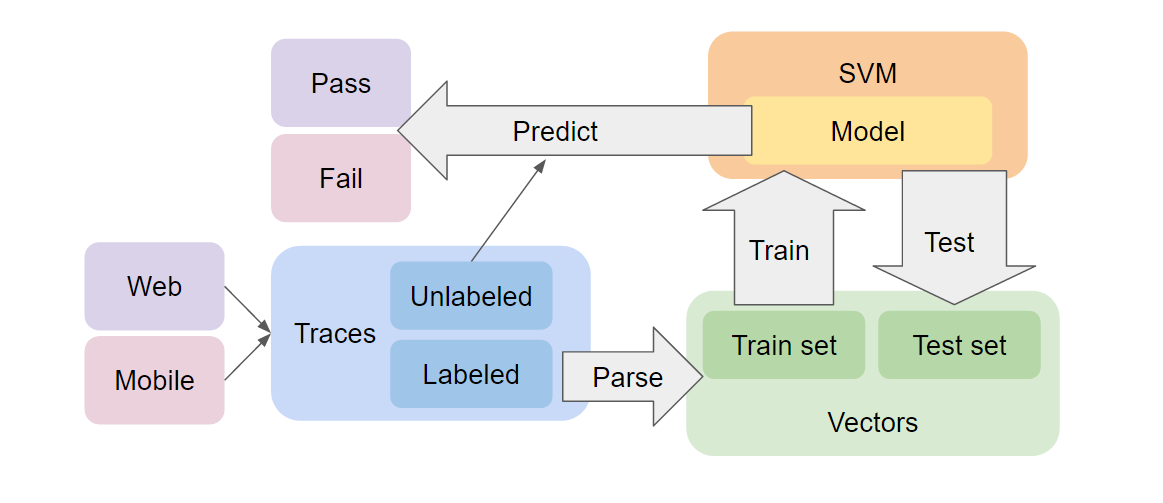
\includegraphics[width=0.8\textwidth]{EvaluateProcedure.png}
	\end{center}
	\caption{ The framework of testing. }
	\label{EvaluateProcedure}
\end{figure}

\clearpage
